\section{Gaussian process surrogate}

The most popular surrogate model is the Gaussian process, which we soon will understand
in more detail. Typically, a probabilistic regression model is on the from 
$$y = f_{\textbf{w}}(x) + \epsilon$$
where weights are trained. $f$ could describe a linear model, $f(x) = \textbf{w}^Tx$ or a polynomial
$f(x) = \sum_i\textbf{w}_i\cdot x_i^2$ etc. %The performance of the regression model is very dependent on how well the data is described in the model. 
The Gaussian process takes a completely different approach; its noisefree prediction\footnote{More
correctly we here mean \textit{predictive distribution}}, $f(x)$, does not depend any parameters
$\textbf{w}$, instead it depends on the vector $\textbf{f} := [f(x_1),\dots,f(x_n)]$ defined on the
input/location data $\textbf{x} = [x_1, \dots, x_n]$. We assign \textbf{f} a multivariate normal distribution, 
$$\textbf{f}|\textbf{x} \sim \mathcal{N}(\bm{\mu}, \bm{\Sigma}),$$
where $\bm{\mu}$ typically is $0$ and the covariance matrix, is dependent on the input, $\textbf{x}$, 
 $$\bm{\Sigma} = c(\textbf{x}, \textbf{x}) = \begin{bmatrix}
    c(x_1,x_1) & \dots & c(x_1,x_n)\\
    \vdots& \ddots\\
    c(x_n,x_1) & \dots & c(x_n,x_n) \end{bmatrix},\hspace{1cm} c(x, y) := Matern(x,y)...$$ this
    means that a realization of the vector $\textbf{f}$ is often close to 0 with a variance of the
    diagonal $\bm{\Sigma}$, but also with a correlation between the elements in $\textbf{f}$ given
    by the off-diagonals in $\bm{\Sigma}$. This is a very important ingredience of a GP, if
    $c(x_1,x_2) \approx 1$ (assuming that the variances of $\textbf{f}$ are 1, then $\bm{\Sigma}$ is
    a \textit{correlation matrix}) then realizations of $\textbf{f}$ always lead to similar values
    of $f(x_1)$ and $f(x_2)$ (this can be seen in Figure \ref{GP_illustration}). This encapsulates
    the idea of a GP: similarities (could be distance or other measures) in $x$ should lead to
    similarities in $f(x)$. Now, in the case of extending it to a regression model, we need to
    introduce the observation $y_*$ for an arbitrary location $x_*$\footnote{The star subscript is
    included to help the reader easily relate $f_*$, $y_*$ and $x_*$.}. Prior to observing any
    data, we assume that the corresponding $f_* = f(x_*)$ is just a new element in the multivariate
    normal distribution, 
\begin{align}\label{prior_gp}
    p(f_*,\textbf{f}|x_*,\textbf{x}) = \mathcal{N}\left(\begin{bmatrix}
        f_*\\ \textbf{f}
    \end{bmatrix} \middle| \begin{bmatrix}
        0\\ \textbf{0}
    \end{bmatrix}, \begin{bmatrix}
        c(x_*, x_*) & c(x_*,\textbf{x})\\
        c(\textbf{x}, x_*) & c(\textbf{x}, \textbf{x})
    \end{bmatrix} \right), 
\end{align}
which yields many possible outcomes for $f_*$ with an average $E[f_*] = 0$ and variance of $V[f_*] =
1$. Note that given a realization of $\textbf{f}$, then the distribution of $f_*$ is changed due to
the correlation $c(x_*, \textbf{x})$. Fortunately, any conditional distribution from a multivariate
normal distribution is easy to deal with. Using appendix \todo{Todo include in appendix} the
conditional distribution of $f_*$ given $\textbf{f}$ is, 
\begin{equation} \label{conditional_GP}
    p(f_*|\textbf{x}, \textbf{f}) = \mathcal{N}(f_*|c(x_*, x_*)^{-1}c(x_*, \textbf{x})\textbf{f},c(x_*, x_*)^{-1}).
\end{equation}
\begin{figure}
    \centering
    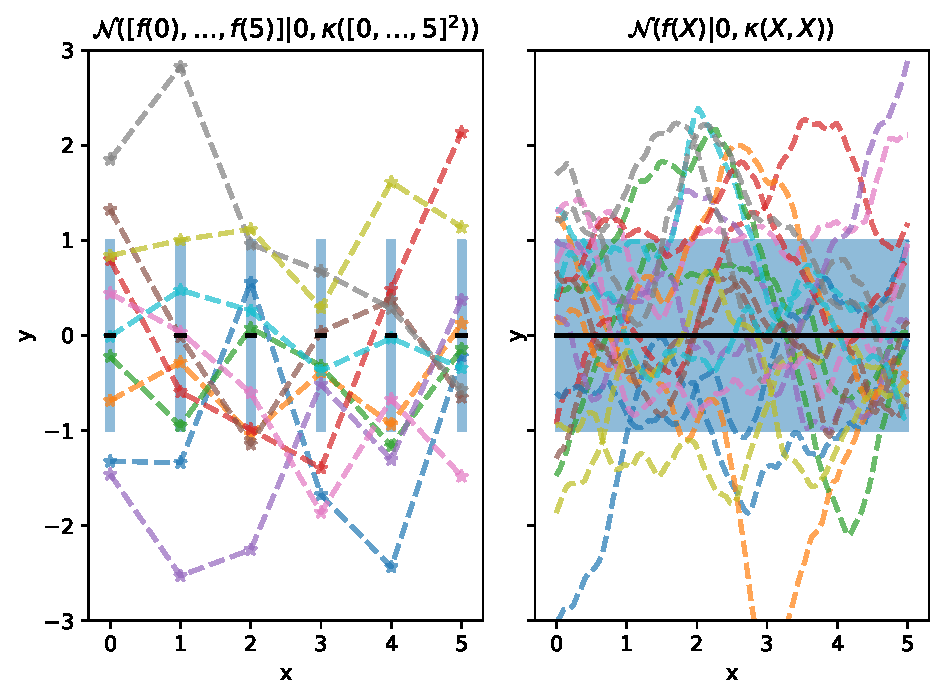
\includegraphics[width = \textwidth]{Pictures/GP_samples_mattern.pdf}
    \caption{Left: Samples from $\mathcal{N}(\textbf{f}|0,\kappa(x_1,\dots, x_{11}))$ where
    $x_i= 0.5(i-1)$. Illustration that a samples from a Gaussian process is just
    samples from the multivariate normal distribution. We could potentially choose
    $\textbf{x}$ to be all of the real line, which will give us the GP - an infinitely
    large multivariate normal distribution (right).}
    \label{GP_illustration}
\end{figure}

\subsection{Exact predictive distribution}
What we want is the predictive posterior distribution, $p(y_*|x_*, \mathcal{D})$, i.e. by
marginalizing out the random variable $f_* := f(x_*)$ (as seen in
\eqref{predictive_posterior_dist}),
\begin{equation}\label{GP_predictive}
    p(y_*|x_*,\mathcal{D}) = \int \mathcal{N}(y_*|f_*, \sigma^2) p(f_*|\mathcal{D})df_*.
\end{equation}
We will soon see that the posterior $p(f_*|\mathcal{D})$ is also a normal distribution 
with mean $\mu_*$ and variance $\sigma^2_*$ so
using \eqref{marginal_distribution} we end up with the closed form Normal distribution, 
$$p(y_*|x_*,\mathcal{D}) = \mathcal{N}(y_*|\mu_*,\sigma^2_*+\sigma^2)$$

So now, we want to calculate $p(f_*|\mathcal{D})$, this can be done using the neat properties of Gaussian
distributions.  
\subsubsection{Posterior function distribution}
From observing the data $\mathcal{D} = \{x_1,y_1, \dots , x_n,y_n\} = (\textbf{x}, \textbf{y})$, we can marginalize over the noisefree
predictions $\textbf{f} = [f(x_1), \dots, f(x_n)]$, 
\begin{equation}\label{posterior_function_new}
    p(f_*|\mathcal{D})= \int p(f_*|\textbf{x}, \textbf{f})p(\textbf{f}|\mathcal{D})d\textbf{f}.
\end{equation} 
From \eqref{conditional_GP} we already have $p(f_*|\textbf{x}, \textbf{f})$ as a Gaussian distribution, so we just need to
calculate the posterior $p(\textbf{f}|\mathcal{D})$, this is done through the prior and likelihood, 
\begin{equation}\label{GP_posterior_unomalized}
    p(\textbf{f}|\mathcal{D}) \propto p(\textbf{f}|\textbf{x}) p(\textbf{y}|\textbf{f}).
\end{equation}
As mentioned $f(\cdot)$ is the noisefree prediction, i.e. $y
= f(x)+ \epsilon$. So assuming iid data, and that $\epsilon$ is additive Gaussian
noise with variance $\sigma^2$, we get the likehood, 
\begin{align*}
    p(\textbf{y}|\textbf{x}, \textbf{f}) = \prod_{i=1}^n p(y_i|x_i,\textbf{f}_i) = \prod_{i=1}^n \mathcal{N}(y_i|\textbf{f}_i,\sigma^2) = \mathcal{N}(\textbf{y}|\textbf{f},\sigma^2 I).
\end{align*}
From \eqref{prior_gp} the prior of $\textbf{f}$ is defined using similarities between its corresponding $\textbf{x}$, giving a
multivariate normal distribution, 
$p(\textbf{f}|\textbf{x}) = \mathcal{N}(\textbf{f}|\textbf{0},c(\textbf{x}, \textbf{x}))$
so we can specify the unomalized posterior \eqref{GP_posterior_unomalized},
\begin{align*}
    p(\textbf{f}|\mathcal{D}) &\propto \mathcal{N}(\textbf{f}|\textbf{0}, c(\textbf{x}, \textbf{x})) \mathcal{N}(\textbf{y}|\textbf{f},\sigma^2 I).
\end{align*}
Noticing that the random quantaties $\textbf{y}$ and $\textbf{f}$ are related such that we can use \eqref{posterior_distribution}, 
we have that the posterior is the following Gaussian: 
\begin{equation*}
    p(\textbf{f}|\mathcal{D}) = \mathcal{N}(\textbf{f}|\Gamma \sigma^{-2}\textbf{y}, \Gamma) \hspace{0.5cm} \Gamma := \left(c(\textbf{x}, \textbf{x})^{-1}+\sigma^{-2} I_n \right)^{-1},
\end{equation*}
where $\Gamma$ is defined according to \eqref{Gamma}. Finally, we see that both terms in the
integral \eqref{posterior_function_new}, are related such that it is possible to use
\eqref{marginal_distribution} \footnote{This can be seen by the relation between $\textbf{f}$ and
$f_*$ in \eqref{posterior_function_new}}, for arriving at, 
\begin{align*}
    p(f_*|\mathcal{D}) &= \mathcal{N}(f_*|\mu_*,\sigma_*^2 )\\
    \mu_* &=  A\Gamma\sigma^{-2}\textbf{y}\\
    \sigma_*^2 &=  c(x_*, x_*)^{-1}+A\Gamma A^T),
\end{align*}
where we define $A :=  c(x_*,x_*)^{-1} c(x_*, \textbf{x})$ agreeing with A in \eqref{marginal_distribution}.
We now have a fully specified Gaussian process posterior function, which we sample from 
in Figure \ref{GP_illustration2}. 


\begin{figure}[h]
    \centering
    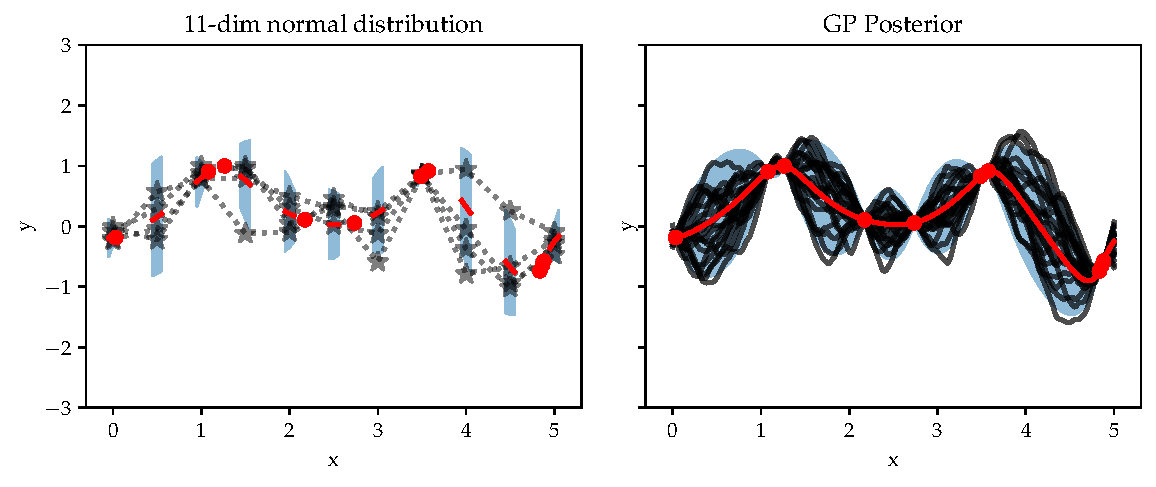
\includegraphics[width = \textwidth]{Pictures/GP2_samples_mattern.pdf}
    \caption{Left: Samples from posterior function distribution for
    $\mathcal{N}(\textbf{f}_*|m(\textbf{x}),V(\textbf{x}))$ where $\textbf{x} = \{x_1,\dots, x_{11}\}$
    and $x_i= 0.5(i-1)$. Illustration that a samples from a Gaussian process is just samples from
    the multivariate normal distribution. We could potentially choose $\textbf{x}$ to be all of the
    real line, which will give us the GP - an infinitely large multivariate normal distribution.}
    \label{GP_illustration2}
\end{figure}



\begin{testexample2}[Trick with normal distributions [from Bishops book?]]
    Given a marginal Gaussian distribution of $x$ and a conditional Gaussian distribution
    of $y$ given $x$ of the form, 
    \begin{align*}
        p(x) &= \mathcal{N}(x|\mu, \Lambda^{-1})\\
        p(y|x) &= \mathcal{N}(y|Ax+b, L^{-1})
    \end{align*}
    then the marginal distribution of $y$ and the conditional distribution of $x$ given $y$
    have the form, 
    \begin{align}
        p(y) &= \mathcal{N}(y|A\mu+b,L^{-1}+A \Lambda^{-1}A^T) \label{marginal_distribution}\\
        p(x|y) &= \mathcal{N}(x|\Gamma \mu+\Gamma [A^TL(y-b)],\Gamma ) \label{posterior_distribution}\\
        \Gamma &:= (\Lambda +A^TLA)^{-1} \label{Gamma}
    \end{align}
\end{testexample2}




\subsection{Learning - Empirical Bayes inference}

The above derivation of the prediction with the Gaussian process only acknowledged $f_*$ as the unknown
variable, however, in \eqref{GP_likelihood} we included the observation variance $\sigma^2$
as the unknown parameter set $\theta$. Additionally, the similarity measurement, which is done in the kernel, 
 $c(\cdot , \cdot )$, is also parameterized. We assumed those additional parameters were known because
of the resulting closed-form predictive posterior. Instead we now call the variance $\sigma^2$ and
kernel parameters hyperparameters. Very often GP hyperparameters are chosen using Emperical bayes, which is simply
to choose the hyperparameters $\nu$, which maximize the marginalized likehood,  
\begin{equation}\label{GP_optim}
    \nu = \argmin_{\nu} p(\textbf{y}|\textbf{x}, \nu)
\end{equation}
where for a Gaussian process the marginal is given as 
\begin{align*}
    p(\textbf{y}|\textbf{x}, \nu) &= \int  p(\textbf{y}, \textbf{f}|\textbf{x}, \nu) d\textbf{f} = \int p(\textbf{y}|\textbf{f},\nu)p(\textbf{f}|\textbf{x},\nu) d\textbf{f},
\end{align*}
where  $p(\textbf{y}|\textbf{f},\nu) = \mathcal{N}(\textbf{y}|\textbf{f},\sigma^2)$ and the prior is
just the Gaussian $p(\textbf{f}|\textbf{x},\nu) = \mathcal{N}(\textbf{f}|0, c_{\nu}(\textbf{x}, \textbf{x}))$
And now we can easily perform the integration using \eqref{marginal_distribution}, 
$$p(\textbf{y}|\textbf{x}, \nu) = \mathcal{N}(\textbf{y}|0,I\sigma^2, c_{\nu}(\textbf{x}, \textbf{x})).$$
Understanding why it makes sense to maximize the marginalized likelihood in order to get the best model
is explained in \cite[165]{bishop}, we will skip this theory, and look at the implications. 

In Figure \ref{GP_two_results} we see that using the same data, the (gradient-based) optimization of \eqref{GP_optim} converge
to two different results, $\log p(y;\nu_1) = -14.29$, and $\log p(y;\nu_2) = -16.70$, and more local optima might exist. Therefore
we optimize the GP with several restarts, when using it as a surrogate model. 

% \todo{Model assessment becomes trivial in light of the model posterior if we
% simply establish preferences over models according to their posterior
% probability. When using the uniform model prior (4.6)
%  the model posterior is proportional to the marginal likelihood alone,
% which can be then used directly for model assessment. ??! Youtube - good video! Go through that!}
\begin{figure}[H]
    \centering
    \begin{minipage}[b]{0.49\textwidth}
     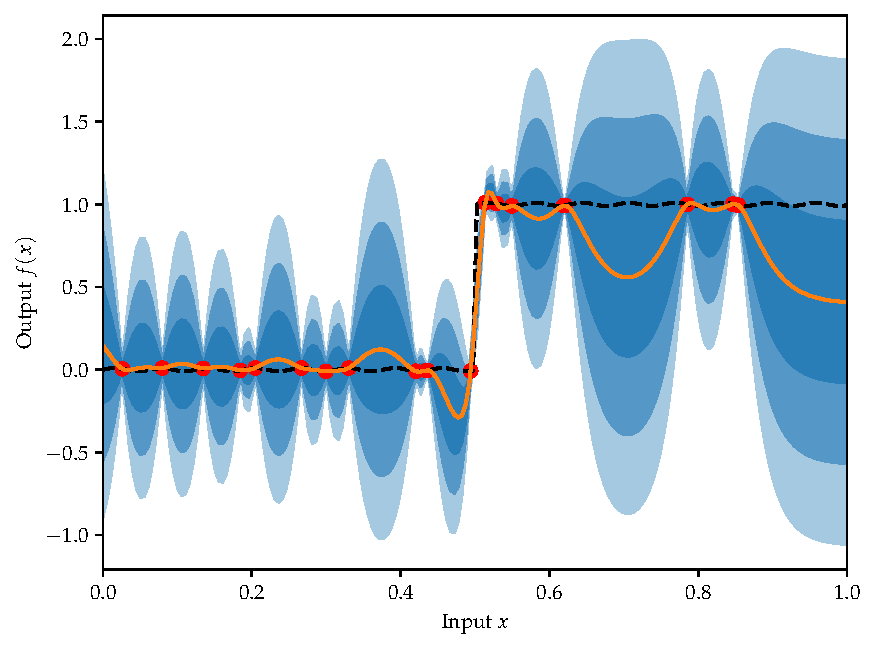
\includegraphics[width=\textwidth]{Pictures/GP_vs_BNN1.pdf}
    \end{minipage}
    \hfill
    \begin{minipage}[b]{0.49\textwidth}
      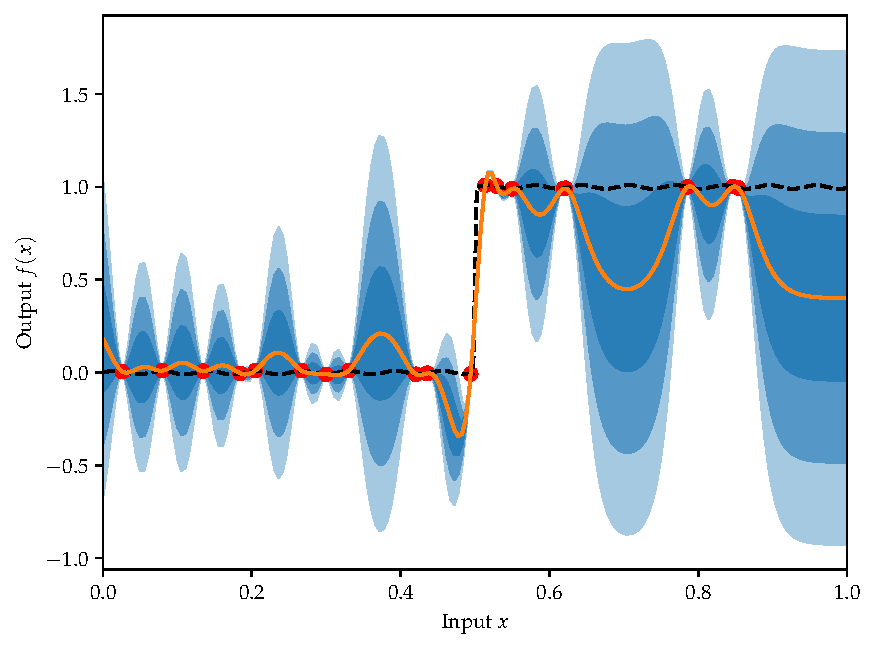
\includegraphics[width=\textwidth]{Pictures/GP_vs_BNN1_b.pdf}
     \end{minipage}
     \caption{The same data fitted with two quite different GPs - note the different lenghtscales in the
     kernel and observation variance $\sigma^2$. Left is chosen 19 out of 20 times and has and marginalized log likelihood of $-16.70$,
     whereas 1 out of 20 runs the solution at right is given with marginalized log likelihood of
     $-14.29$.}
     \label{GP_two_results}
\end{figure}
